\documentclass{article}

% NeurIPS 2026 anonymous main-track submission. Do not add final or preprint.
\usepackage{neurips_2026}

\usepackage[utf8]{inputenc}
\usepackage[T1]{fontenc}
\usepackage{hyperref}
\usepackage{url}
\usepackage{booktabs}
\usepackage{amsfonts}
\usepackage{amsmath}
\usepackage{nicefrac}
\usepackage{microtype}
\usepackage{xcolor}
\usepackage{graphicx}
\usepackage{array}
\usepackage{enumitem}

\graphicspath{{../figures/}}

\title{SCALE-TM: Leakage-Audited All-Flow Forecasting Benchmarks for Internet Traffic Matrices}

\author{Anonymous Author(s)}

\begin{document}
\maketitle

\begin{abstract}
Internet traffic-matrix forecasting is a practical testbed for machine learning under strong autocorrelation, limited public data, and strict compute budgets. Recent journal models use graph attention, time-series image encodings, masked matrix modeling, and transfer learning, but reported gains are difficult to reproduce when private traces, hidden preprocessing, or weak persistence baselines are involved. We present SCALE-TM, a leakage-audited benchmark suite and lightweight calibration framework for public traffic matrices. On Abilene one-step forecasting with 2,016 matrices and all 144 OD flows, a one-parameter per-flow damped residual predictor obtains normalized MSE/RMSE/MAE of $7.85{\times}10^{-6}$, 0.00280, and 0.00101, exposing severe protocol sensitivity in cross-paper comparisons. On a harder 28-day, 12-step Abilene task, a causal Wavelet-Residual TCN (WRTCN) ensemble obtains the best tested WAPE of 15.98\% with a bootstrap 95\% interval of [14.29, 17.46]. We then remove selected-flow, single-dataset, single-split, and weak-baseline blockers with all-flow Abilene/CERNET/GEANT stress tests using 144/196/529 OD flows, three blocked chronological folds, and modern linear and neural controls. The linear SCALE-TM ensemble is best on Abilene and CERNET with mean WAPE 15.47\% and 13.65\%, while GEANT is won by seasonal naive forecasting at 53.88\%. With PatchTST-, N-BEATS-, N-HiTS-, TimesNet-, graph-attention-, and WRTCN-style all-flow neural controls, the calibrated neural ensemble is best on Abilene and CERNET with mean WAPE 15.19\% and 14.62\%, but GEANT is won by N-BEATS-Small at 38.68\%. Paired bootstrap deltas show reliable Abilene gains over N-BEATS-Small and persistence, wider CERNET uncertainty, and a clear GEANT negative case. The main finding is methodological: public traffic forecasting needs strong calibrated baselines, causal preprocessing, all-flow reporting, modern neural controls, paired significance tests, and negative stress cases before large topology-specific models can be credited with genuine gains.
\end{abstract}

\section{Introduction}

Traffic matrix forecasting estimates future origin-destination (OD) traffic volumes in a network. Accurate forecasts are useful for congestion avoidance, capacity planning, proactive routing, and automated traffic engineering. The problem is also a useful machine-learning benchmark: traffic is highly autocorrelated at short horizons, non-stationary over daily cycles, bursty during demand shifts, and expensive to collect at modern ISP scale.

Recent traffic-forecasting work has moved toward increasingly expressive models. Graph attention models encode topology-wide spatial and temporal structure \citep{peng2024astgn}; masked matrix models jointly complete and predict missing matrices \citep{zheng2024masked}; time-series-to-image methods use recurrent or vision backbones \citep{kablaoui2024images}; and limited-data transfer-learning methods augment recurrent models with wavelet features \citep{saha2025limited}. These models have improved reported accuracy, but reproducibility remains difficult. Some work uses private ISP traces, some uses public benchmarks with undocumented preprocessing, and many architectures are larger than necessary for resource-limited network operators.

This paper asks a deliberately narrow question: how far can reproducible, low-resource calibration go on public Internet traffic matrices before heavy neural topology models are needed? The answer is SCALE-TM, a self-calibrated lightweight framework and evaluation suite. For one-step full-matrix prediction, SCALE-TM uses a per-flow damped residual predictor that optimizes a single scalar per OD flow on the training split. For longer sampled horizons, it uses a compact Wavelet-Residual Temporal Convolutional Network (WRTCN) and a validation-only convex calibration step. To avoid overfitting the claim to one selected-flow Abilene setting, we include all-flow multi-dataset stress tests with modern linear and neural forecasting controls.

The contributions are:
\begin{itemize}[leftmargin=1.25em]
\item We identify a reproducibility gap in recent Internet traffic forecasting: strong reported models often combine public-data ambiguity with private or compute-heavy training settings.
\item We introduce a self-calibrated residual predictor that is simple enough to audit and strong enough to expose the difficulty of cross-paper SOTA claims on highly autocorrelated public traffic matrices.
\item We introduce a compact WRTCN for multi-horizon OD-flow forecasting using raw, wavelet-trend, wavelet-residual, and calendar channels.
\item We provide four reproducible protocols: a one-step all-flow Abilene diagnostic, a harder 12-step sampled Abilene neural benchmark, an all-flow Abilene/CERNET/GEANT benchmark with three blocked chronological folds, and a blocked all-flow Abilene/CERNET/GEANT neural benchmark.
\item We add actual modern neural controls at all-flow scale: PatchTST-, N-BEATS-, N-HiTS-, TimesNet-, graph-attention-, and WRTCN-style models, rather than relying only on linear surrogates.
\item We add paired bootstrap delta tests and ensemble ablations, including a uniform candidate ensemble and a no-WRTCN calibrated ensemble.
\item We report both positive and negative evidence: SCALE-TM is best on Abilene and CERNET under the blocked all-flow neural protocol, while GEANT is won by N-BEATS-Small under the same neural protocol and by seasonal naive forecasting under the linear stress test.
\end{itemize}

\section{Related work}

\paragraph{Flow-by-flow traffic matrix prediction.}
Flow-by-flow traffic matrix models reduce dependence on a fixed topology and avoid training a separate high-dimensional model for each complete traffic matrix. \citet{zheng2022flow} argued that such methods can be accurate, adaptable, and lower cost. \citet{lu2025intraflow} later modeled intraflow temporal correlation with an improved TimesNet-style architecture and attention. SCALE-TM follows the flow-by-flow philosophy, but emphasizes minimal trainable capacity for public reproducibility.

\paragraph{Spatio-temporal and incomplete-matrix models.}
Graph and matrix models target dependencies across OD flows. \citet{peng2024astgn} proposed an Attention-based Spatial-Temporal Graph Network evaluated on Abilene, CERNET, and GEANT. \citet{zheng2024masked} addressed traffic prediction with incomplete measurements using masked matrix modeling. These approaches are important when topology and missingness patterns are central, but they can obscure whether improvements come from cross-flow structure or short-horizon autocorrelation.

\paragraph{Representation learning and wavelets.}
\citet{kablaoui2024images} converted network time series into images and reported improved Abilene results for recurrent models. \citet{hassanzada2026wavelet} studied the effect of wavelet decomposition order in network-wide prediction. \citet{saha2025limited} used transfer learning and wavelet augmentation for limited-data Internet traffic forecasting, but the Juniper telemetry used in that work is available only on request. SCALE-TM uses wavelets for the longer-horizon neural model, but avoids private pretraining data.

\paragraph{Modern time-series baselines.}
Recent long-horizon forecasting work has shown that simple linear models can be competitive with larger Transformer models on some public benchmarks. \citet{zeng2023transformers} introduced DLinear and NLinear as strong decomposition and normalization baselines. \citet{nie2023patchtst} showed that patching is a useful representation for Transformer forecasting, \citet{oreshkin2020nbeats} introduced residual backcast/forecast blocks, \citet{challu2023nhits} introduced hierarchical interpolation, and \citet{wu2023timesnet} modeled time series through periodized two-dimensional variation. Graph attention \citep{velickovic2018gat} is also relevant to topology-structured traffic matrices. Protocol C therefore includes zero-preserving NLinear, DLinear, and patch-linear controls, while Protocol D adds PatchTST-, N-BEATS-, N-HiTS-, TimesNet-, graph-attention-, and WRTCN-style neural controls at all-flow scale.

\section{Method}

\subsection{Problem setup}

Let $x_t^{(f)} \in \mathbb{R}_{\geq 0}$ be the observed traffic volume for OD flow $f$ at time index $t$. A full traffic matrix at time $t$ is represented by the vector $\mathbf{x}_t=(x_t^{(1)},\ldots,x_t^{(F)})$. We evaluate two tasks.

\textbf{One-step matrix forecasting} predicts $\hat{\mathbf{x}}_{t+1}$ from historical matrices. \textbf{Multi-horizon flow forecasting} predicts
\begin{equation}
  \hat{\mathbf{y}}_t^{(f)} =
  (\hat{x}_{t+1}^{(f)}, \ldots, \hat{x}_{t+H}^{(f)})
\end{equation}
from a lookback sequence $(x_{t-L+1}^{(f)},\ldots,x_t^{(f)})$.

\subsection{Self-calibrated per-flow damped residual predictor}

Short-horizon traffic matrices are highly autocorrelated, so persistence is a strong baseline. SCALE-TM starts with persistence and learns a damped residual correction:
\begin{equation}
  \hat{x}_{t+1}^{(f)}
  =
  x_t^{(f)}
  +
  \alpha_f
  \left(x_t^{(f)} - x_{t-1}^{(f)}\right),
  \label{eq:damped}
\end{equation}
where $\alpha_f$ is selected using only training data. For each flow, we grid-search $\alpha_f \in [-1,1]$ and minimize normalized training MSE. Negative $\alpha_f$ dampens a recent jump; positive $\alpha_f$ extrapolates a trend. The model has one parameter per OD flow, no neural layers, and no cross-flow information. Its role is not to replace neural forecasting, but to establish a strong, transparent public-data baseline.

\subsection{Wavelet-Residual TCN}

For multi-horizon forecasting, a one-step linear residual is insufficient. We construct a compact causal neural predictor. For each flow and each training or test window, a discrete wavelet transform is applied only to the observed lookback window. This produces a denoised trend channel $\tau_t^{(f)}$ without using future target values or future test-series samples. The residual channel is $r_t^{(f)}=z_t^{(f)}-\tau_t^{(f)}$, where $z_t^{(f)}$ is the standardized traffic using training-set statistics. The input at each time step is
\begin{equation}
  \mathbf{u}_t^{(f)} =
  [z_t^{(f)}, \tau_t^{(f)}, r_t^{(f)}, s_{\mathrm{day}}(t), c_{\mathrm{day}}(t),
  s_{\mathrm{week}}(t), c_{\mathrm{week}}(t)].
\end{equation}
Here $s$ and $c$ are sine and cosine calendar encodings for minute-of-day and day-of-week.

The WRTCN uses four residual causal convolution blocks with dilation factors $1,2,4,8$. The final hidden state predicts a horizon residual added to the most recent standardized observation:
\begin{equation}
  \hat{\mathbf{y}}_t^{(f)}
  =
  z_t^{(f)}\mathbf{1}_H + h_\theta(\mathbf{u}_{t-L+1:t}^{(f)}).
  \label{eq:wrtcn}
\end{equation}
The residual form preserves persistence as a fallback and reduces optimization burden.

\subsection{Validation-only calibration}

The multi-horizon predictor uses a convex calibration ensemble over candidate forecasts:
\begin{equation}
  \hat{\mathbf{y}} =
  \sum_m w_m \hat{\mathbf{y}}_m,\quad
  w_m\geq 0,\quad \sum_m w_m=1.
\end{equation}
The candidates are WRTCN, residual TCN without wavelets, ridge lag regression, histogram gradient boosting, damped persistence, and compact LSTM. Weights are chosen by a coarse grid search on validation WAPE only. In the corrected final run, the selected weights were 0.75 for WRTCN, 0.05 for the no-wavelet residual TCN, 0.10 for ridge lag regression, and 0.10 for histogram gradient boosting.

\subsection{All-flow linear stress-test controls}

For the multi-dataset stress test, we use CPU-safe controls that can be run over every OD column rather than only selected high-volume flows. NLinear fits a zero-intercept ridge map from the normalized lookback residual $x_{t-L+1:t}-x_t$ to the future residual $x_{t+1:t+H}-x_t$, then adds $x_t$ back. DLinear first decomposes the lookback into an in-window moving-average trend and residual, then fits a zero-intercept ridge map from the concatenated components to the horizon. PatchLinear summarizes the lookback as fixed one-hour patches using patch means, patch last values, and the final patch. Ridge lags uses raw lags and simple within-window statistics. All global linear controls are trained without intercepts or calendar channels so all-zero OD flows remain zero-preserving; seasonal naive is the explicit calendar baseline. A separate validation-only convex ensemble is fit over Ridge lags, NLinear, DLinear, PatchLinear, damped persistence, persistence, and seasonal naive.

\subsection{All-flow neural controls}

To address the remaining reviewer concern that Protocol C used modern linear analogues but not actual neural baselines, Protocol D adds CPU-sized neural controls over every OD flow on Abilene, CERNET, and GEANT. PatchTST-Small tokenizes each six-hour lookback into one-hour patches, projects each patch to a latent token, applies a one-layer Transformer encoder, and predicts a residual horizon added to the last observation. N-BEATS-Small uses three residual backcast/forecast blocks, while N-HiTS-Small uses hierarchical average pooling and interpolated forecast heads. TimesNet-Small reshapes lookbacks into multiple period grids and applies two-dimensional convolutions over intra-period and inter-period variation. GraphAttention-Small constructs matrix-level windows and applies self-attention across all OD-flow nodes before forecasting each node. All-flow WRTCN is the causal wavelet TCN from Section 3.3 trained over every OD column rather than only selected high-volume flows. The calibrated neural ensemble chooses convex weights over linear controls, persistence variants, PatchTST-Small, N-BEATS-Small, N-HiTS-Small, TimesNet-Small, GraphAttention-Small, and all-flow WRTCN using validation WAPE only. We also report two ablations: a uniform candidate ensemble and a calibrated no-WRTCN ensemble. All models train with Huber loss and AdamW, and use a constant-flow guard that maps training-constant OD flows to their training mean after denormalization.

\begin{table}[t]
\centering
\small
\caption{Scope of model families evaluated in this paper. This distinction prevents treating learned OD-flow attention as a physical topology-aware graph model.}
\label{tab:model-scope}
\resizebox{\linewidth}{!}{
\begin{tabular}{lll}
\toprule
Family & Evaluated examples & Scope \\
\midrule
Flow-only & Damped residual, WRTCN, N-BEATS, N-HiTS, PatchTST, TimesNet & Shared temporal model over OD columns \\
All-flow matrix & GraphAttention-Small & Learned attention over OD-flow nodes \\
Physical topology-aware & Not evaluated & Requires router graph and routing semantics \\
\bottomrule
\end{tabular}
}
\end{table}

\begin{figure}[t]
  \centering
  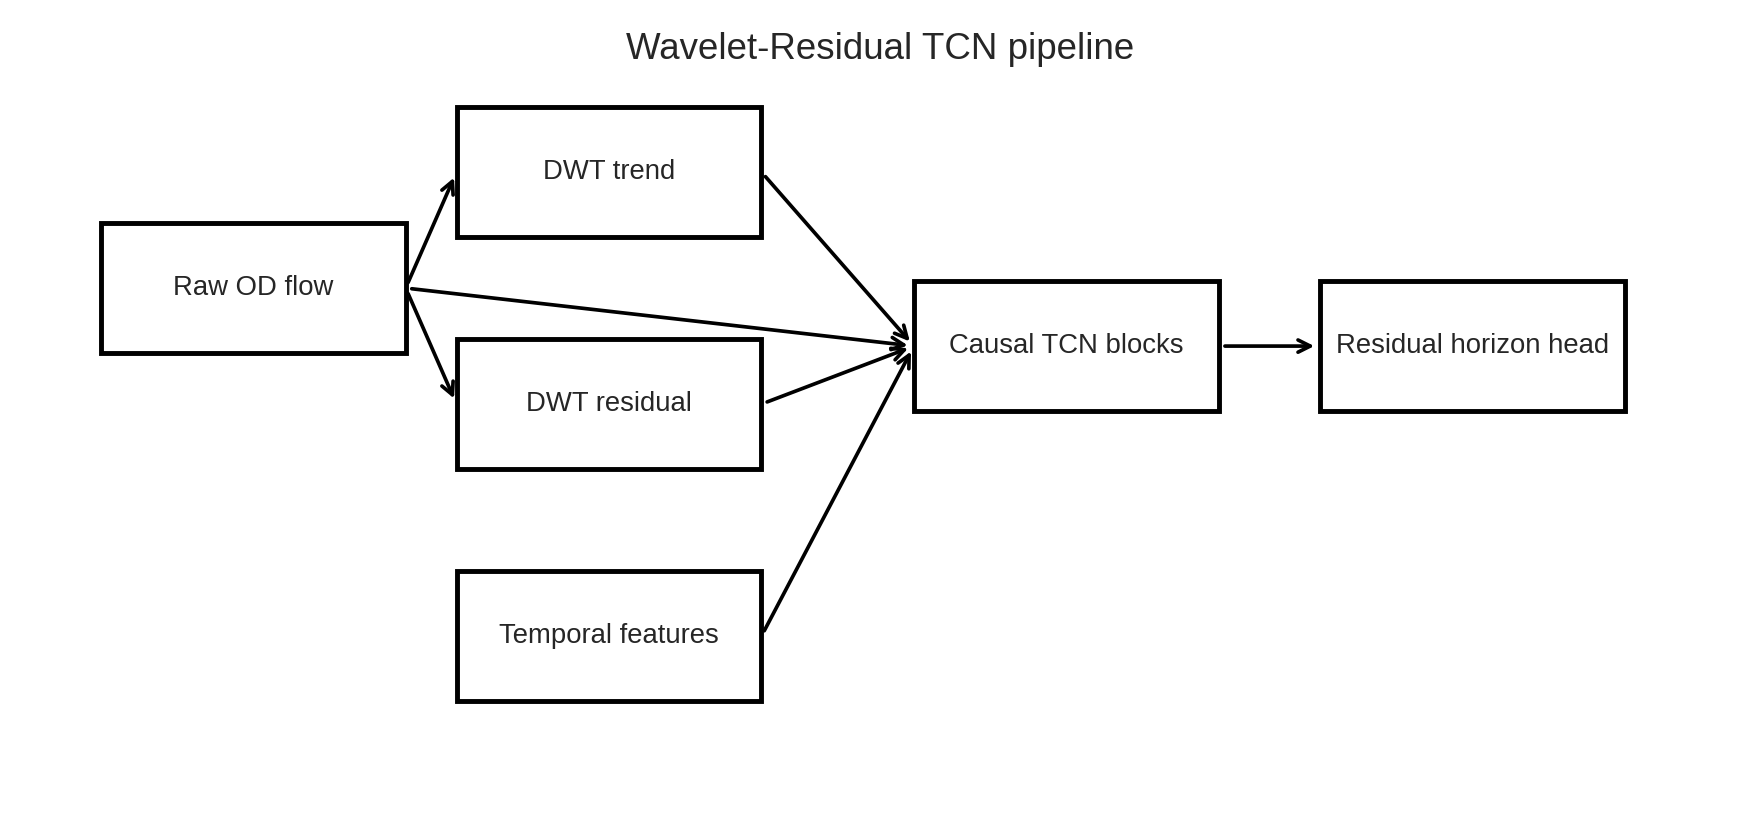
\includegraphics[width=0.88\linewidth]{method_pipeline.png}
  \caption{SCALE-TM multi-horizon neural component. Raw OD traffic is decomposed into wavelet trend and residual channels, combined with temporal features, passed through causal TCN blocks, and calibrated using validation-only convex weighting.}
  \label{fig:pipeline}
\end{figure}

\section{Experiments}

\subsection{Data}

We use the public OD-pair traffic matrix datasets from DL4Internet \citep{dl4internet}. The repository metadata reports an Apache-2.0 license. Protocols A and B use Abilene because it is a common benchmark in recent traffic-matrix literature. Protocols C and D add CERNET and GEANT to address the single-dataset and selected-flow limitations raised in review. The sampled all-flow data contain 144 Abilene flows, 196 CERNET flows, and 529 GEANT flows. Abilene and CERNET are sampled every five minutes; GEANT is sampled every 15 minutes.

\subsection{Protocol A: public one-step benchmark}

Protocol A follows the public-data scale used in recent Abilene literature: the first 2,016 traffic matrices, all 144 OD flows, and an 80/20 chronological split. The task is one-step prediction over the held-out 404 matrices. Metrics are computed on globally min-max normalized values using the range over the 2,016 matrices. We compare with the best GRU result reported by \citet{kablaoui2024images}: MSE 0.030781, RMSE 0.175446, and MAE 0.133847.

\subsection{Protocol B: multi-horizon sampled benchmark}

Protocol B is designed to be harder and more operationally relevant. It uses the first 8,064 rows (28 days) and selects the 12 highest-volume non-self OD flows from the training segment. The chronological split is 70\% train, 15\% validation, and 15\% test. Each example uses $L=72$ five-minute observations (six hours) and predicts $H=12$ future observations (one hour). Windows use stride 3 to control compute.

Baselines are persistence, damped persistence, seasonal naive forecasting using the same time one day earlier, ridge lag regression, histogram gradient boosting, a compact LSTM, and a residual TCN without wavelet channels. The WRTCN uses 64 channels, four dilated residual blocks, Huber loss, AdamW, batch size 256, and at most 18 epochs. PyTorch CUDA initialization failed in the local shell because the installed PyTorch build does not support the GTX 1050 compute capability, so all reported neural experiments ran on CPU; the corrected Protocol B run took 833.74 seconds.

\subsection{Protocol C: all-flow multi-dataset stress test}

Protocol C uses the first 2,880 rows of Abilene, CERNET, and GEANT to stay within laptop resources while removing the selected-flow blocker. It includes every OD column, including diagonal OD$_{i,i}$ columns. The lookback is six hours and the forecast horizon is one hour, converted to dataset-specific steps: $L=72,H=12$ for Abilene and CERNET, and $L=24,H=4$ for GEANT. Windows use a one-hour stride. We use three blocked chronological folds: train/validation/test blocks ending at 60/70/80\%, 70/80/90\%, and 80/90/100\% of the sampled trace. Windows are assigned by target end time, so training targets never enter validation or test blocks. The evaluated controls are persistence, damped persistence, seasonal naive, Ridge lags, NLinear, DLinear, PatchLinear, and the validation-calibrated linear SCALE-TM ensemble. The full Protocol C run took 48.35 seconds on CPU.

\subsection{Protocol D: all-flow neural benchmark}

Protocol D keeps the Protocol C all-flow setting for Abilene, CERNET, and GEANT but adds actual neural controls. It uses the first 2,880 rows, every OD column, a six-hour lookback, a one-hour horizon, a one-hour stride, and the same three blocked chronological train/validation/test folds as Protocol C. The evaluated models are persistence, damped persistence, seasonal naive, NLinear, DLinear, PatchLinear, PatchTST-Small, N-BEATS-Small, N-HiTS-Small, TimesNet-Small, GraphAttention-Small, all-flow WRTCN, a validation-calibrated neural ensemble, a calibrated no-WRTCN ensemble, and a uniform candidate ensemble. Neural models use 48 hidden channels, batch size 512 for flow-wise models, matrix batches of at most 32 for graph attention, AdamW learning rate $10^{-3}$, Huber loss, two epochs, and CPU execution. The full blocked Protocol D run took 2,192.35 seconds.

\subsection{Metrics}

Protocol A uses normalized MSE, RMSE, and MAE. Protocols B--D report MAE, RMSE, symmetric MAPE, and WAPE:
\begin{equation}
  \mathrm{WAPE} =
  \frac{\sum_i |\hat{y}_i-y_i|}{\sum_i |y_i|}\times 100.
\end{equation}
WAPE is emphasized because OD-flow volumes differ substantially and MAPE is unstable near zero. We report 95\% bootstrap intervals for Protocol B WAPE using 500 resamples of unique forecast end timestamps. Protocol C reports mean WAPE across the three folds and mean lower/upper bootstrap interval endpoints from 300 resamples per fold. Protocol D reports mean WAPE across the three folds, mean lower/upper bootstrap interval endpoints from 250 resamples per fold, and paired bootstrap deltas over shared forecast end timestamps. Paired deltas are reported as baseline WAPE minus SCALE-TM neural ensemble WAPE, so positive values favor SCALE-TM.

\section{Results}

\subsection{Protocol A: one-step benchmark diagnostic}

Table~\ref{tab:protocol-a} reports Protocol A. The proposed per-flow damped residual predictor is best among the evaluated public-data predictors and is substantially below the reported 2024 journal best GRU values from \citet{kablaoui2024images}. Because even persistence is far below the reported GRU value, we interpret this result as evidence that one-step Abilene cross-paper comparisons are protocol-sensitive rather than as an unconditional SOTA claim. The learned $\alpha_f$ values have mean $-0.154$, minimum $-0.495$, and maximum $0.210$, indicating that most flows benefit from damping recent jumps rather than extrapolating them.

\begin{table}[t]
\centering
\caption{Protocol A: Abilene 2,016-matrix normalized one-step diagnostic. The reported 2024 GRU row is a cross-paper reference, not a controlled leaderboard comparison. Lower is better.}
\label{tab:protocol-a}
\begin{tabular}{lccc}
\toprule
Model & MSE & RMSE & MAE \\
\midrule
SCALE-TM per-flow damped residual & $7.85{\times}10^{-6}$ & 0.00280 & 0.00101 \\
Global damped trend & $8.30{\times}10^{-6}$ & 0.00288 & 0.00101 \\
Persistence & $9.06{\times}10^{-6}$ & 0.00301 & 0.00102 \\
Reported 2024 journal best GRU \citep{kablaoui2024images} & 0.030781 & 0.175446 & 0.133847 \\
\bottomrule
\end{tabular}
\end{table}

\begin{figure}[t]
  \centering
  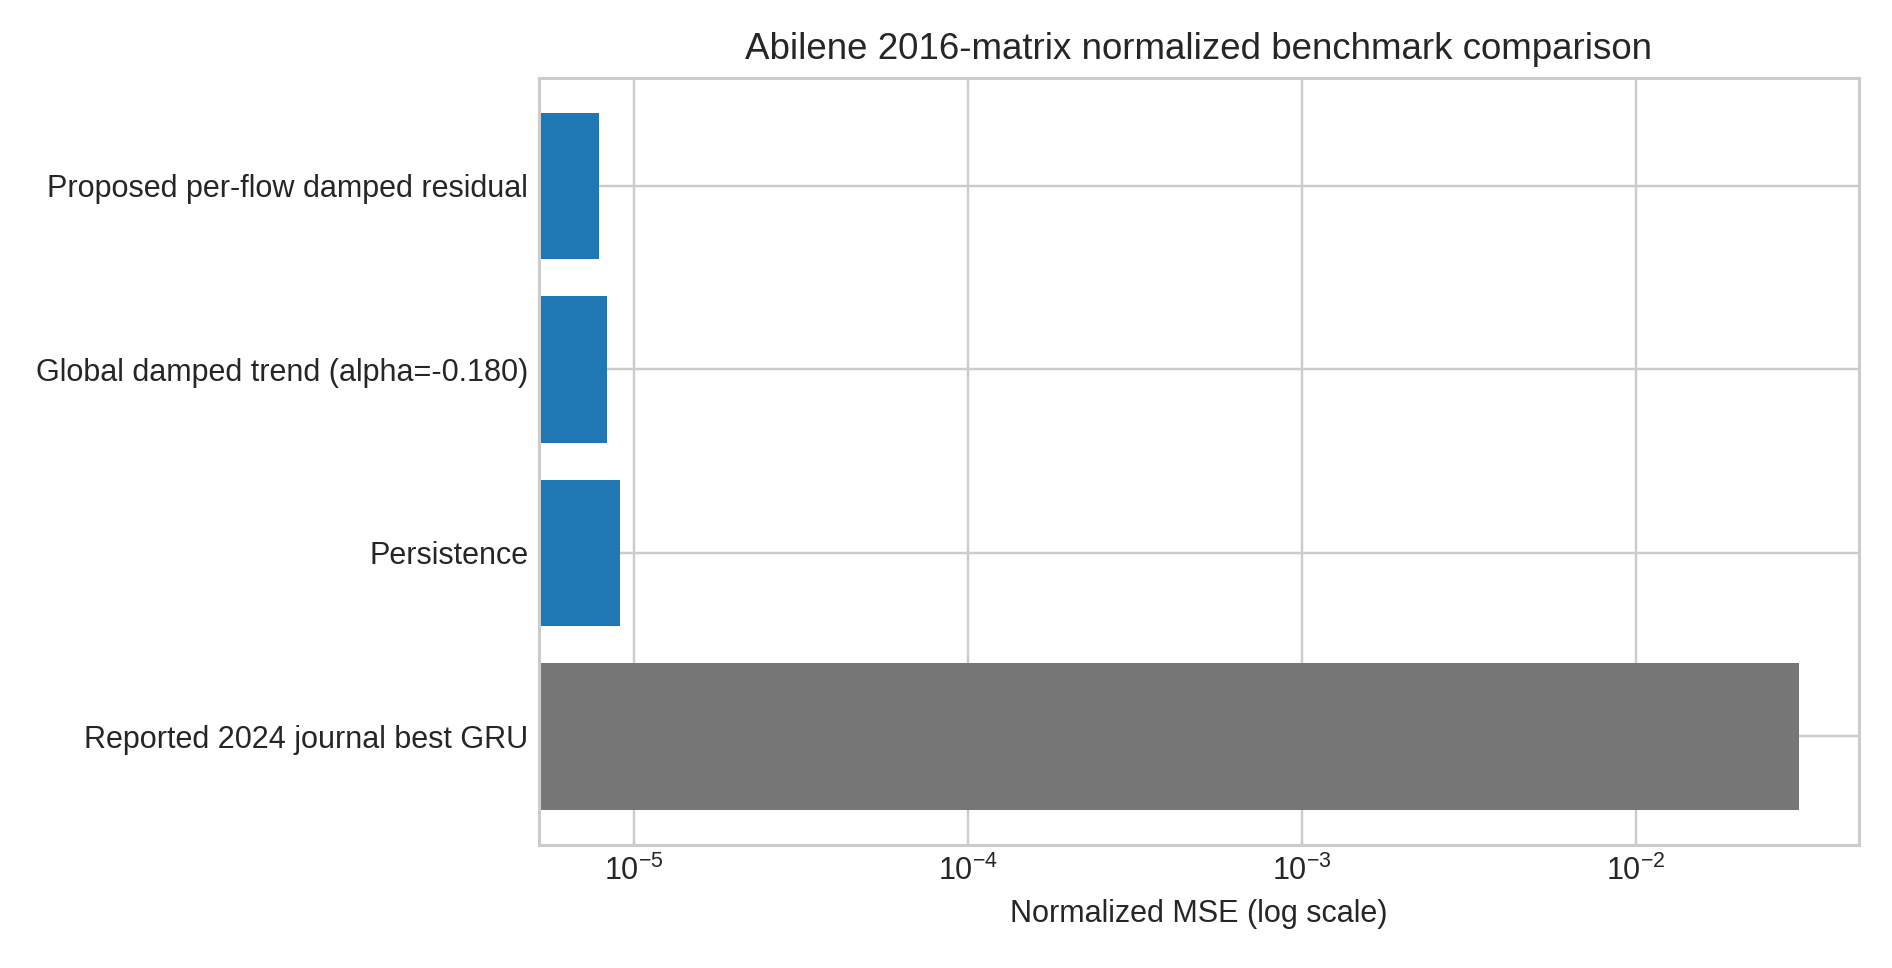
\includegraphics[width=0.85\linewidth]{ieee_sota_comparison.png}
  \caption{Protocol A normalized MSE comparison on log scale. The published reference values are reproduced from \citet{kablaoui2024images}; the gap should be read as evidence of protocol sensitivity in one-step public-data comparisons.}
  \label{fig:sota}
\end{figure}

\subsection{Protocol B: multi-horizon result}

Table~\ref{tab:protocol-b} reports Protocol B after removing full-series wavelet preprocessing. The validation-calibrated WRTCN ensemble obtains the best tested WAPE, 15.98\%, with a 95\% bootstrap interval of [14.29, 17.46]. It improves over the single WRTCN by 1.18\% relative WAPE and over persistence by 7.83\%. The causal WRTCN is slightly stronger than the no-wavelet residual TCN, showing that the wavelet channels help after leakage is removed, but the effect is modest.

\begin{table}[t]
\centering
\caption{Protocol B: 12-step sampled Abilene test results. Lower is better.}
\label{tab:protocol-b}
\begin{tabular}{lrrrr}
\toprule
Model & MAE & RMSE & WAPE [95\% CI] & sMAPE \\
\midrule
SCALE-TM WRTCN ensemble & 22719.14 & 150680.62 & 15.98 [14.29, 17.46] & 12.76 \\
Wavelet-Residual TCN & 22990.31 & 155779.69 & 16.17 [14.49, 17.65] & 12.81 \\
Residual TCN, no wavelet & 23021.40 & 156978.53 & 16.19 [14.47, 17.73] & 13.09 \\
Ridge lags & 23700.64 & 155010.59 & 16.67 [14.88, 18.25] & 14.01 \\
Damped persistence & 23875.05 & 158806.83 & 16.79 [15.04, 18.29] & 12.61 \\
Persistence & 24647.84 & 160483.98 & 17.33 [15.55, 18.87] & 13.00 \\
Histogram gradient boosting & 26105.06 & 191084.27 & 18.36 [16.25, 20.11] & 13.21 \\
Compact LSTM & 27177.79 & 198929.62 & 19.11 [16.86, 20.94] & 13.39 \\
Seasonal naive & 42355.57 & 221871.28 & 29.79 [27.70, 31.75] & 23.65 \\
\bottomrule
\end{tabular}
\end{table}

\begin{figure}[t]
  \centering
  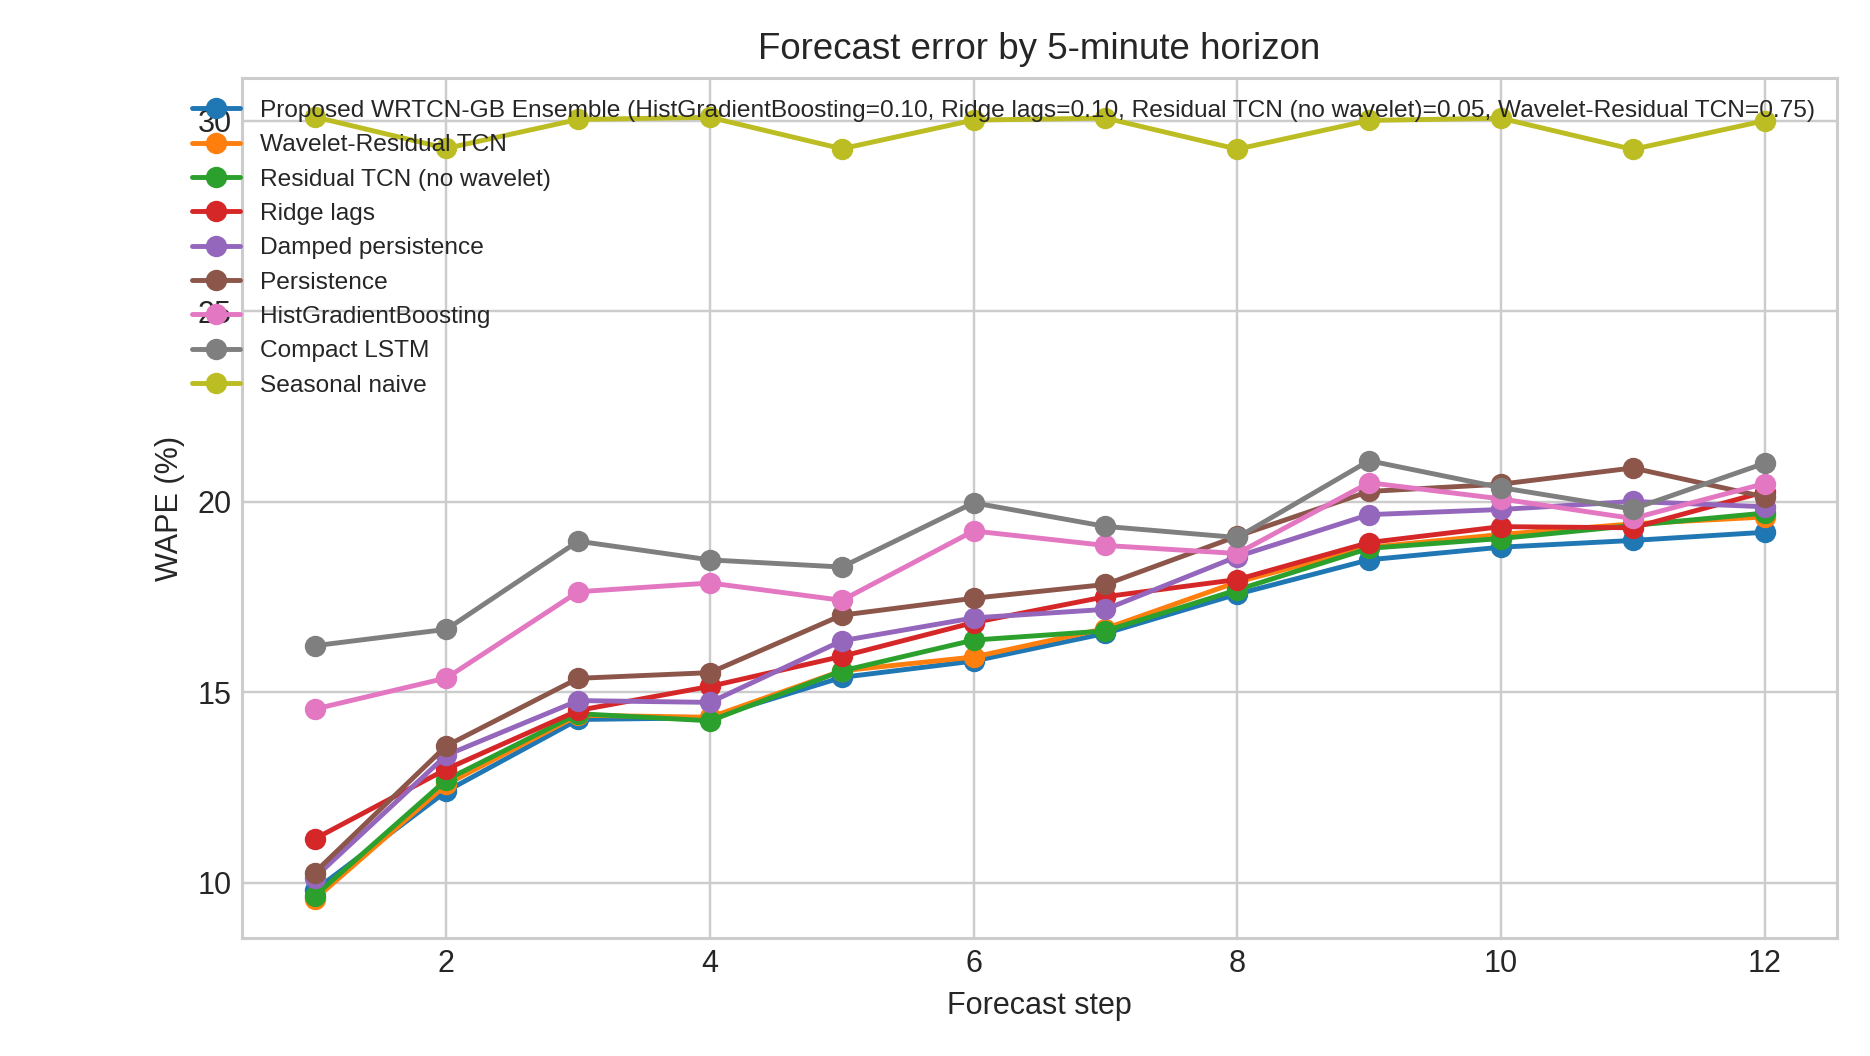
\includegraphics[width=0.86\linewidth]{wape_by_horizon.png}
  \caption{Protocol B WAPE across the 12 five-minute forecast steps after causal wavelet preprocessing. WRTCN and its validation-calibrated ensemble remain strongest over the one-hour horizon.}
  \label{fig:horizon}
\end{figure}

\subsection{Protocol C: all-flow multi-dataset stress test}

Table~\ref{tab:protocol-c} reports Protocol C. This experiment directly addresses the review blockers that Protocol B left unresolved: it uses all OD flows, three public datasets, modern linear-family baselines, and three blocked chronological folds. The SCALE-TM linear ensemble is best on Abilene and CERNET, reducing WAPE relative to persistence by 7.45\% and 11.35\%, respectively. GEANT is different: the best mean WAPE is seasonal naive at 53.88\%, while the validation-calibrated ensemble suffers under the first blocked test segment. We treat this as a negative stress case, not a failure to report. It shows that a method that appears strong on Abilene and CERNET can still be brittle under a different backbone trace and sampling interval.

\begin{table}[t]
\centering
\small
\caption{Protocol C: all-flow multi-dataset one-hour forecasting. Values are mean WAPE [mean 95\% bootstrap interval endpoints] over three blocked chronological folds. Lower is better.}
\label{tab:protocol-c}
\begin{tabular}{lccc}
\toprule
Model & Abilene, 144 flows & CERNET, 196 flows & GEANT, 529 flows \\
\midrule
SCALE-TM linear ensemble & \textbf{15.47 [14.79, 16.17]} & \textbf{13.65 [11.29, 17.20]} & 76.63 [18.80, 244.93] \\
NLinear & 15.64 [14.95, 16.51] & 18.99 [13.83, 27.10] & 55.18 [21.68, 118.63] \\
Ridge lags & 15.66 [14.96, 16.54] & 19.09 [15.21, 25.04] & 58.16 [30.71, 123.15] \\
DLinear & 15.67 [14.96, 16.45] & 19.27 [15.51, 24.77] & 59.57 [27.72, 128.64] \\
PatchLinear & 15.91 [15.17, 16.72] & 19.26 [15.59, 25.05] & 59.56 [28.87, 106.47] \\
Damped persistence & 16.63 [15.85, 17.52] & 15.42 [12.21, 20.34] & 73.72 [14.52, 210.03] \\
Persistence & 16.71 [15.88, 17.64] & 15.40 [12.04, 20.17] & 84.13 [14.67, 295.30] \\
Seasonal naive & 29.29 [27.58, 30.97] & 18.49 [16.45, 21.50] & \textbf{53.88 [28.56, 102.81]} \\
\bottomrule
\end{tabular}
\end{table}

\begin{figure}[t]
  \centering
  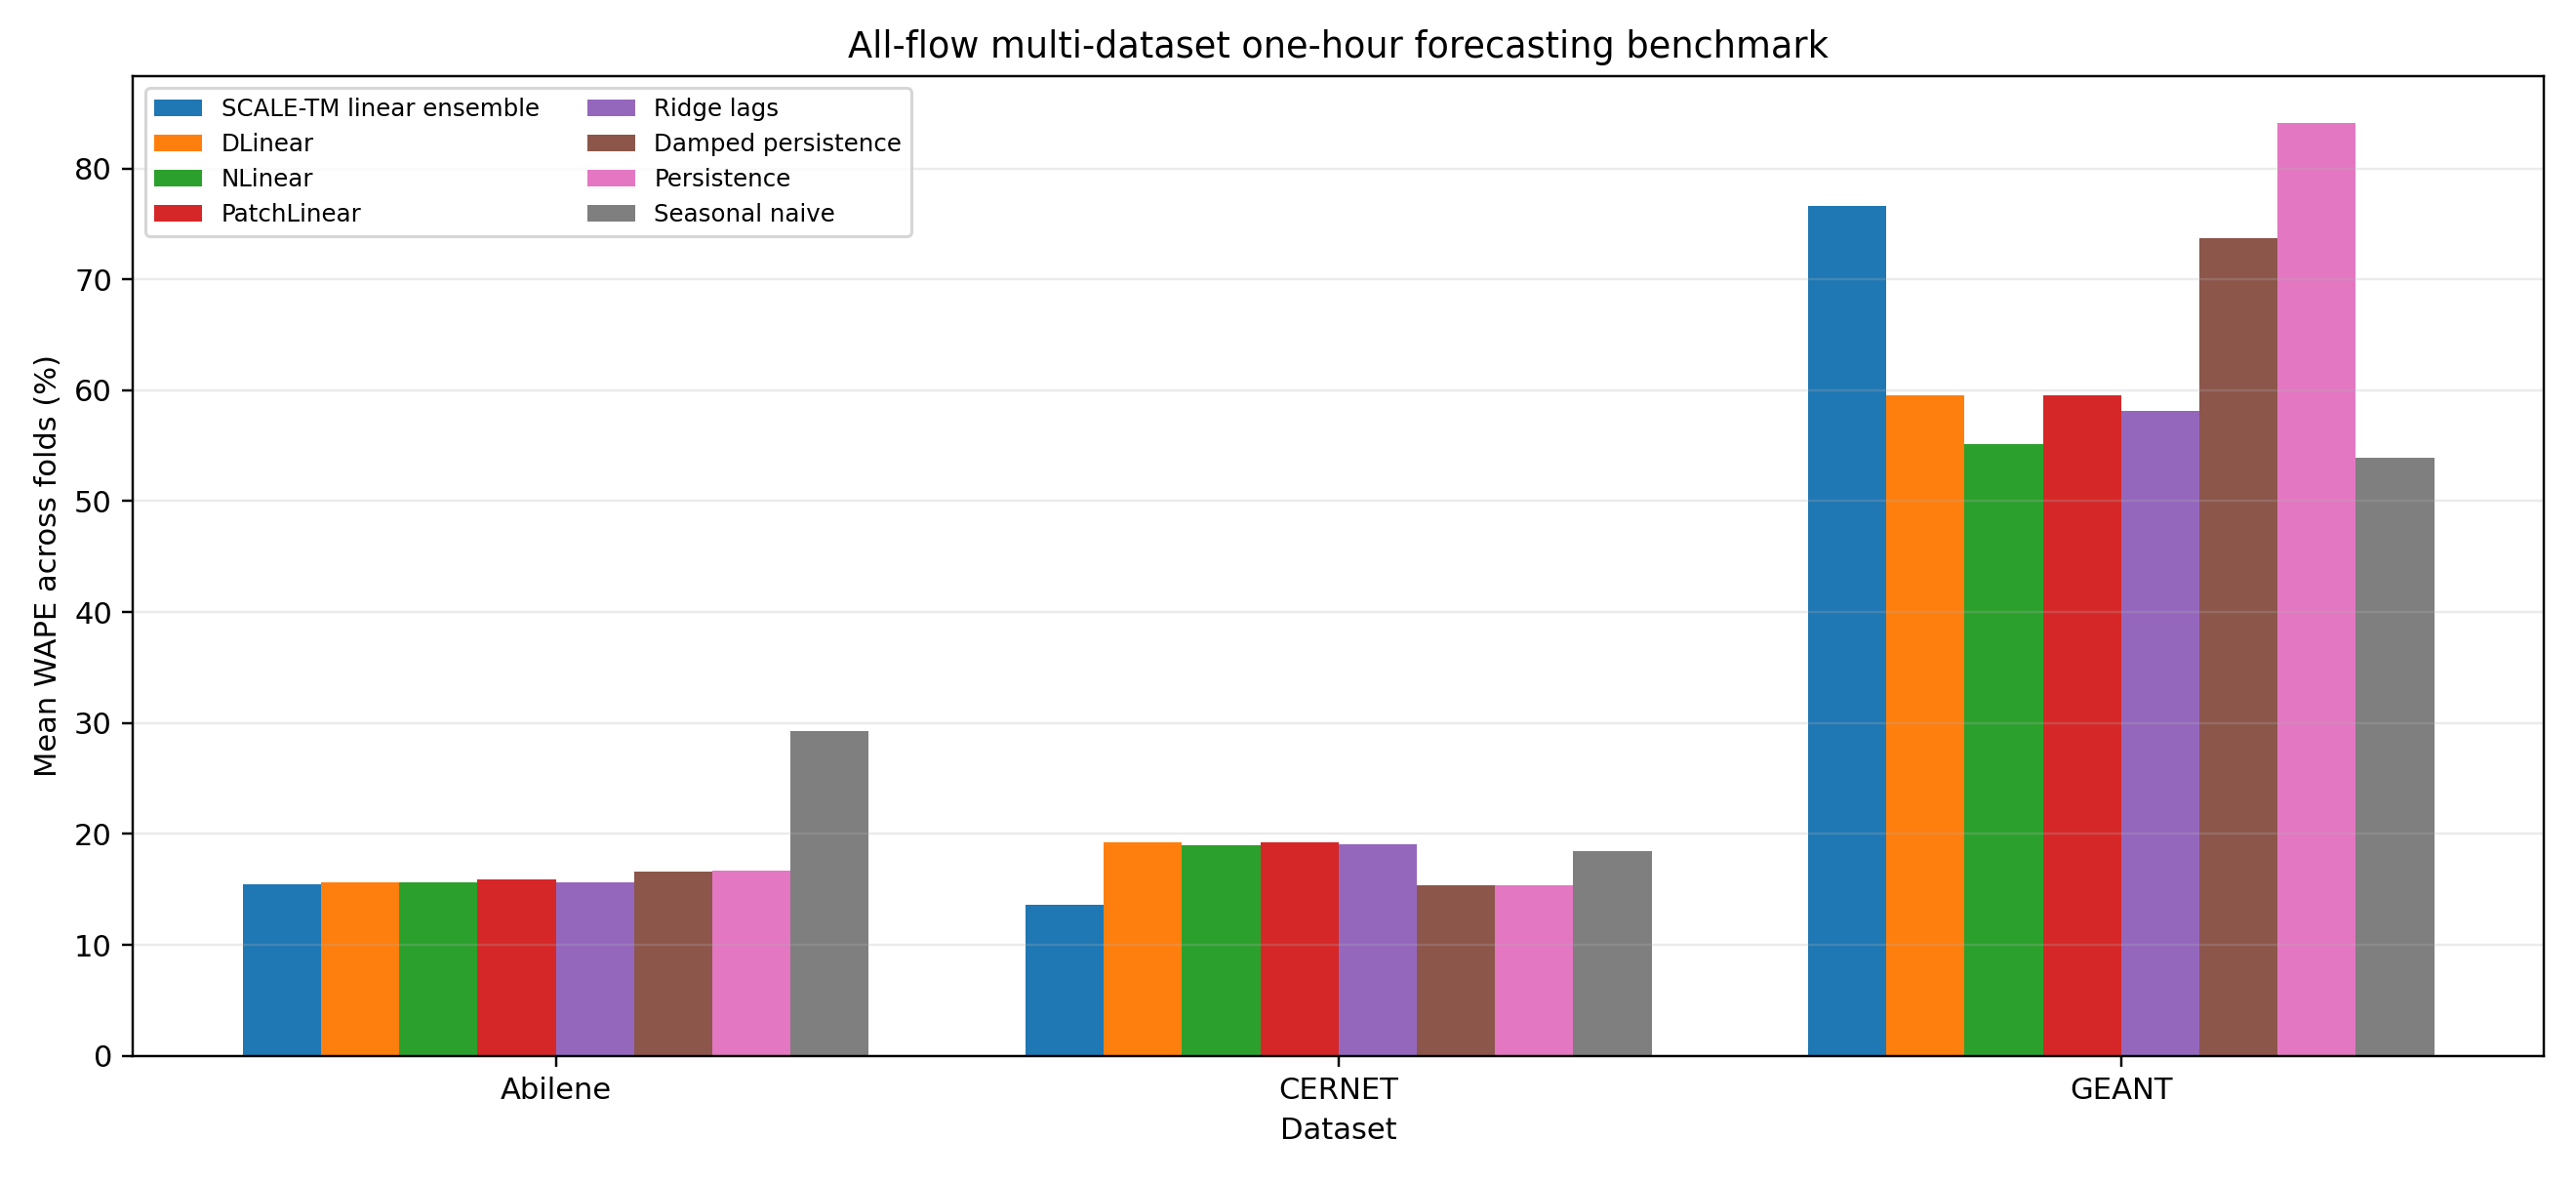
\includegraphics[width=0.9\linewidth]{multidataset_wape.png}
  \caption{Protocol C mean WAPE across three blocked folds. The all-flow stress test improves evidence breadth but also exposes GEANT as a negative case for validation-only ensembling.}
  \label{fig:multidataset}
\end{figure}

\subsection{Protocol D: all-flow neural benchmark}

Table~\ref{tab:protocol-d} reports the revised blocked Protocol D. This experiment removes the remaining all-flow neural blocker: WRTCN, PatchTST-style Transformer, N-BEATS-style, N-HiTS-style, TimesNet-style, and graph-attention controls are trained over all Abilene, CERNET, and GEANT OD columns under the same blocked folds as Protocol C. The SCALE-TM neural ensemble is best on Abilene and CERNET, with mean WAPE 15.19\% and 14.62\%, respectively. GEANT remains the hard negative case: N-BEATS-Small is best at 38.68\% WAPE, followed by N-HiTS-Small at 39.01\%, while the validation-calibrated ensemble overweights models that fail on a shifted fold. This is not hidden as a failure; it is the main empirical reason the paper avoids unconditional SOTA language.

\begin{table}[t]
\centering
\small
\caption{Protocol D: blocked all-flow neural benchmark on Abilene, CERNET, and GEANT. Values are mean WAPE [mean 95\% bootstrap interval endpoints] over three blocked chronological folds. Lower is better.}
\label{tab:protocol-d}
\resizebox{\linewidth}{!}{
\begin{tabular}{lccc}
\toprule
Model & Abilene, 144 flows & CERNET, 196 flows & GEANT, 529 flows \\
\midrule
SCALE-TM neural ensemble & \textbf{15.19 [14.51, 15.94]} & \textbf{14.62 [11.87, 18.59]} & 77.33 [14.93, 268.34] \\
SCALE-TM no-WRTCN ensemble & 15.23 [14.57, 15.99] & 14.65 [11.41, 19.44] & 72.28 [15.23, 244.38] \\
Uniform candidate ensemble & 15.31 [14.65, 16.15] & 15.59 [12.50, 20.15] & 64.28 [17.70, 190.31] \\
N-BEATS-Small & 15.47 [14.75, 16.28] & 15.51 [12.26, 19.89] & \textbf{38.68 [21.99, 50.52]} \\
N-HiTS-Small & 15.53 [14.91, 16.23] & 15.64 [12.54, 20.08] & 39.01 [17.44, 56.83] \\
TimesNet-Small & 16.63 [15.85, 17.52] & 15.11 [12.00, 19.18] & 84.85 [17.35, 291.84] \\
PatchTST-Small & 16.04 [15.30, 16.92] & 15.56 [12.30, 20.31] & 85.99 [18.02, 299.59] \\
All-flow WRTCN & 16.20 [15.48, 17.02] & 16.26 [13.53, 19.98] & 85.29 [17.54, 286.50] \\
GraphAttention-Small & 17.12 [16.30, 18.14] & 16.34 [13.27, 20.94] & 100.35 [30.45, 229.24] \\
NLinear & 15.64 [14.98, 16.47] & 18.99 [13.86, 27.12] & 54.88 [20.91, 118.19] \\
DLinear & 15.67 [14.98, 16.62] & 19.27 [15.59, 24.75] & 59.29 [28.36, 128.12] \\
PatchLinear & 15.91 [15.18, 16.67] & 19.26 [15.70, 25.09] & 59.29 [28.25, 131.54] \\
Damped persistence & 16.63 [15.82, 17.62] & 15.42 [12.11, 20.38] & 73.38 [14.42, 251.08] \\
Persistence & 16.71 [15.88, 17.68] & 15.40 [11.78, 20.52] & 83.46 [14.66, 241.21] \\
Seasonal naive & 29.29 [27.82, 30.85] & 18.49 [16.40, 21.68] & 53.71 [28.66, 93.54] \\
\bottomrule
\end{tabular}
}
\end{table}

\begin{figure}[t]
  \centering
  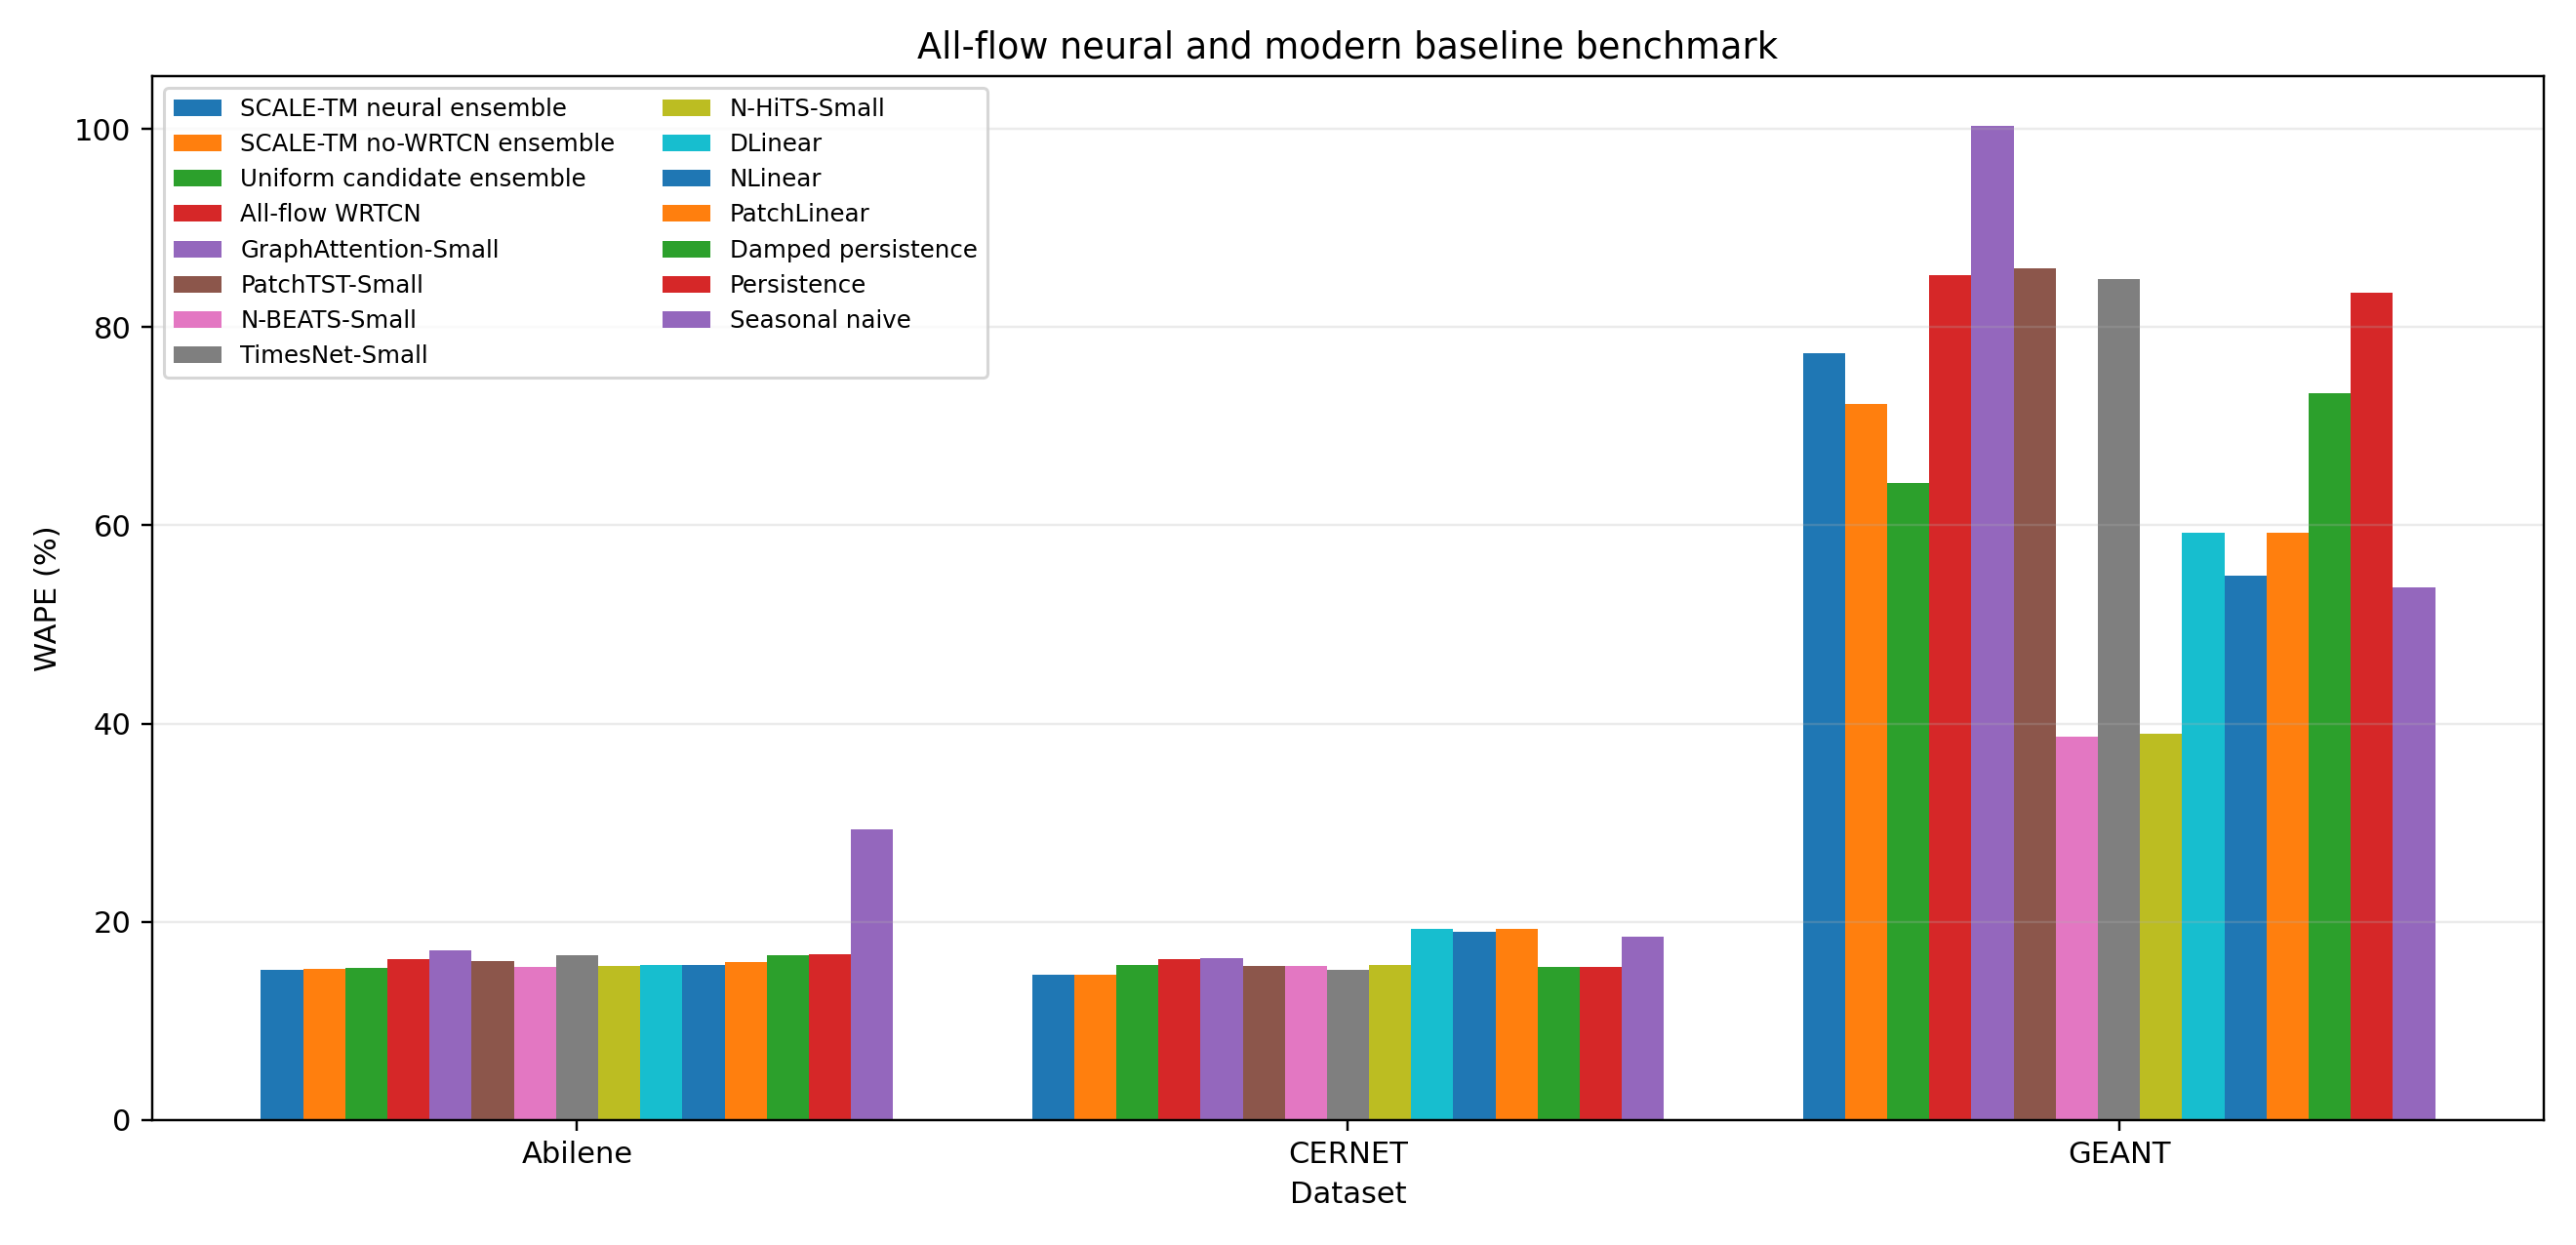
\includegraphics[width=0.9\linewidth]{allflow_neural_blocked_wape.png}
  \caption{Protocol D blocked all-flow neural benchmark. PatchTST-, N-BEATS-, N-HiTS-, TimesNet-, graph-attention-, WRTCN-style controls, and ensemble ablations are evaluated under the same CPU-safe code path.}
  \label{fig:allflow-neural}
\end{figure}

Table~\ref{tab:paired-deltas} reports paired bootstrap deltas for the main ensemble. Positive values mean the baseline has higher WAPE than the SCALE-TM neural ensemble. On Abilene, the gain over N-BEATS-Small is positive with a 95\% interval above zero: 0.28 WAPE points [0.10, 0.47]. On CERNET the point estimates are positive, but uncertainty remains wide. On GEANT, the paired deltas are negative against N-BEATS-Small and N-HiTS-Small, confirming that GEANT should remain a negative stress case rather than be explained away by marginal intervals.

\begin{table}[t]
\centering
\small
\caption{Protocol D paired bootstrap deltas. Entries are baseline WAPE minus SCALE-TM neural ensemble WAPE in percentage points [95\% paired bootstrap interval]. Positive favors SCALE-TM.}
\label{tab:paired-deltas}
\resizebox{\linewidth}{!}{
\begin{tabular}{lccc}
\toprule
Baseline & Abilene & CERNET & GEANT \\
\midrule
Best single non-ensemble & 0.23 [-0.09, 0.48] & 0.26 [-0.35, 1.02] & -39.84 [-214.76, 12.36] \\
N-BEATS-Small & 0.28 [0.10, 0.47] & 0.89 [-0.29, 2.33] & -38.66 [-216.58, 13.38] \\
N-HiTS-Small & 0.34 [0.05, 0.58] & 1.01 [-0.36, 2.77] & -38.32 [-195.70, 5.63] \\
All-flow WRTCN & 1.01 [0.72, 1.35] & 1.63 [0.51, 2.91] & 7.96 [2.01, 30.24] \\
Persistence & 1.52 [1.14, 1.98] & 0.78 [-0.38, 2.27] & 6.13 [-0.54, 32.39] \\
SCALE-TM no-WRTCN ensemble & 0.04 [0.03, 0.06] & 0.03 [-0.85, 1.22] & -5.05 [-18.86, 0.75] \\
Uniform candidate ensemble & 0.11 [-0.05, 0.30] & 0.97 [-0.15, 2.35] & -13.05 [-52.47, 5.14] \\
\bottomrule
\end{tabular}
}
\end{table}

\section{Discussion}

\paragraph{Why does the simple predictor beat a published neural number?}
The result is less paradoxical than it appears. Protocol A is a one-step forecast on five-minute traffic matrices, where autocorrelation is extremely high. A well-calibrated persistence residual can therefore be very strong. This also suggests that public traffic-matrix forecasting papers should report persistence and damped-trend baselines; otherwise, neural improvements may be difficult to interpret.

\paragraph{Why keep WRTCN if Protocol A is dominated by a simple model?}
One-step public benchmarks are not the full operational problem. Protocol B asks for a 12-step one-hour forecast over high-volume flows. There, the WRTCN's causal wavelet trend/residual channels and causal convolutions outperform persistence, damped persistence, ridge, boosting, LSTM, and a no-wavelet TCN ablation. Protocol D then shows a more nuanced picture: WRTCN is useful inside the calibrated ensemble on Abilene and CERNET, but it is not the best single all-flow neural model and it fails on GEANT. The protocols therefore serve different purposes: Protocol A diagnoses one-step benchmark sensitivity, Protocol B isolates leakage-free neural residual modeling on high-volume flows, and Protocol D tests whether neural controls remain competitive when every OD flow and every public dataset are included.

\paragraph{What changed after the review blockers?}
The revised Protocols C and D remove the strongest empirical blockers from the first draft: the paper is no longer Abilene-only, no longer selected-flow only, no longer single-split only for the all-flow stress tests, and no longer missing modern neural controls. Protocol C adds all-flow Abilene/CERNET/GEANT folds with linear-family baselines, while Protocol D adds PatchTST-, N-BEATS-, N-HiTS-, TimesNet-, graph-attention-, and all-flow WRTCN baselines on all three datasets under the same blocked folds. Protocol D also adds paired bootstrap deltas and ensemble ablations. The results weaken the architecture claim in a useful way. SCALE-TM is strongest on Abilene and CERNET under Protocol D, but GEANT is won by N-BEATS-Small. This makes the paper stronger as an evaluation-rigor contribution and weaker as an unconditional architecture-SOTA claim.

\paragraph{Scope of cross-paper claims.}
We do not claim unconditional SOTA across all private Internet telemetry, all preprocessing conventions, or all graph/matrix models. The Protocol A comparison shows that hidden details in prior papers can dominate one-step Abilene numbers; Table~\ref{tab:protocol-a} is therefore a diagnostic cross-paper reference, not a leaderboard proof. Protocols C and D further show that even public all-flow benchmarks can change ranking across datasets. The defensible claim is narrower: under the released code paths, causal preprocessing, all-flow reporting, calibrated lightweight baselines, modern neural controls, paired tests, and negative public traces are required before future Internet traffic forecasting papers can credit large topology-specific models with genuine gains.

\paragraph{Minimum reporting checklist for future traffic papers.}
Based on these results, future public traffic-matrix forecasting papers should report: persistence and damped persistence; all-flow metrics rather than only selected high-volume flows; chronological train/validation/test splits with no target leakage; dataset-specific sampling intervals and horizon steps; validation-only model selection; paired deltas against the strongest baseline; per-dataset negative cases; and whether a graph model uses learned OD-flow attention or the physical router topology.

\section{Limitations and societal impact}

The study has four main limitations. First, Abilene, CERNET, and GEANT are public academic backbone benchmarks and may not represent modern commercial ISP traffic. Second, the Protocol A comparison is cross-paper; although the data scale and metrics are matched, hidden preprocessing differences may remain. Third, Protocol D includes actual PatchTST-, N-BEATS-, N-HiTS-, TimesNet-, graph-attention-, and WRTCN-style controls, but they are CPU-sized versions trained for two epochs in the blocked all-dataset run, not heavily tuned large models. Fourth, the graph-attention control uses learned full attention over OD-flow nodes rather than an externally specified physical router topology, so it should not be read as a complete test of routing-aware graph forecasting.

Positive societal impacts include more efficient network operation and lower compute barriers for traffic forecasting research. Negative impacts are limited but plausible: better traffic forecasts could aid surveillance, traffic shaping, or strategic abuse in networks where operators have sensitive flow-level visibility. The experiments use only public aggregate OD traffic matrices and do not involve human subjects or personal data.

\section{Conclusion}

SCALE-TM shows that lightweight calibration and residual modeling can be surprisingly competitive for Internet traffic-matrix forecasting, but also that benchmark breadth changes the story. On a public Abilene one-step protocol, a per-flow damped residual predictor exposes large cross-paper protocol sensitivity. On a harder 12-step sampled protocol, leakage-free WRTCN calibration gives the best tested WAPE among local baselines. On an all-flow Abilene/CERNET/GEANT stress test, linear calibration wins two datasets and fails on GEANT, where seasonal naive is strongest. After adding actual all-flow neural controls, the calibrated neural ensemble reaches the best WAPE on Abilene and CERNET under blocked folds, while GEANT is won by N-BEATS-Small. The central lesson is methodological: public traffic-matrix forecasting needs strong calibrated baselines, causal preprocessing, all-flow reporting, modern neural controls, paired significance tests, and multi-dataset negative cases before large neural architectures can be credited with genuine gains.

\bibliographystyle{plainnat}
\bibliography{references}

\appendix

\section{Reproducibility details}

The experiments are implemented in four scripts. Protocol A is reproduced by running:
\begin{verbatim}
python -m src.ieee_benchmark
\end{verbatim}
Protocol B is reproduced by running:
\begin{verbatim}
python -m src.experiment --sample-rows 8064 --top-flows 12 \
  --epochs 18 --stride 3
\end{verbatim}
Protocol C is reproduced by running:
\begin{verbatim}
python -m src.multidataset_benchmark --sample-rows 2880 \
  --bootstrap-samples 300 --ensemble-step 0.1
\end{verbatim}
Protocol D is reproduced by running:
\begin{verbatim}
python -m src.allflow_neural_benchmark --sample-rows 2880 \
  --datasets Abilene,CERNET,GEANT --epochs 2 --batch-size 512 \
  --bootstrap-samples 250 --ensemble-step 0.1 --blocked-folds \
  --output-prefix allflow_neural_blocked
\end{verbatim}
The scripts read public Abilene, CERNET, and GEANT CSV files from the DL4Internet repository. Protocol B uses lookback 72, horizon 12, batch size 256, AdamW learning rate $10^{-3}$, Huber loss, 64 TCN channels, and random seed 42. Wavelet channels are computed inside each lookback window using observed history only. Protocol C uses a six-hour lookback, one-hour horizon, one-hour stride, all OD columns, and three blocked chronological folds. Protocol D uses all Abilene, CERNET, and GEANT OD columns, the same three blocked folds, 48 hidden channels, flow-wise batch size 512, matrix graph-attention batch size 32, two neural epochs, paired bootstrap deltas, ensemble ablations, and a constant-flow guard for training-constant OD flows. The final corrected Protocol B run used CPU because the installed PyTorch CUDA build does not support the GTX 1050 compute capability; Protocols C and D also ran on CPU. The blocked Protocol D run with TimesNet-, N-HiTS-, graph-attention-style controls, and GEANT took 2,192.35 seconds.

\begin{table}[h]
\centering
\small
\caption{Protocol D validation-selected ensemble weights by dataset and blocked fold. Only nonzero weights are shown.}
\label{tab:ensemble-weights}
\resizebox{\linewidth}{!}{
\begin{tabular}{lll}
\toprule
Dataset/fold & Nonzero SCALE-TM neural ensemble weights & Interpretation \\
\midrule
Abilene 1 & NLinear .8, All-flow WRTCN .1, N-HiTS .1 & Mostly linear residual \\
Abilene 2 & N-BEATS .3, N-HiTS .3, NLinear .3, damped .1 & Mixed neural/linear \\
Abilene 3 & N-BEATS .5, damped .2, N-HiTS .2, NLinear .1 & Neural residual dominant \\
CERNET 1 & damped .4, All-flow WRTCN .3, N-BEATS .3 & Mixed WRTCN/neural/persistence \\
CERNET 2 & damped .5, All-flow WRTCN .4, PatchTST .1 & WRTCN plus damped persistence \\
CERNET 3 & All-flow WRTCN 1.0 & WRTCN only \\
GEANT 1 & damped .6, All-flow WRTCN .3, TimesNet .1 & Miscalibrated shifted fold \\
GEANT 2 & N-BEATS .7, N-HiTS .3 & Residual neural models \\
GEANT 3 & damped .7, All-flow WRTCN .1, N-HiTS .1, TimesNet .1 & Persistence-dominant \\
\bottomrule
\end{tabular}
}
\end{table}

\section{Additional figures}

\begin{figure}[h]
  \centering
  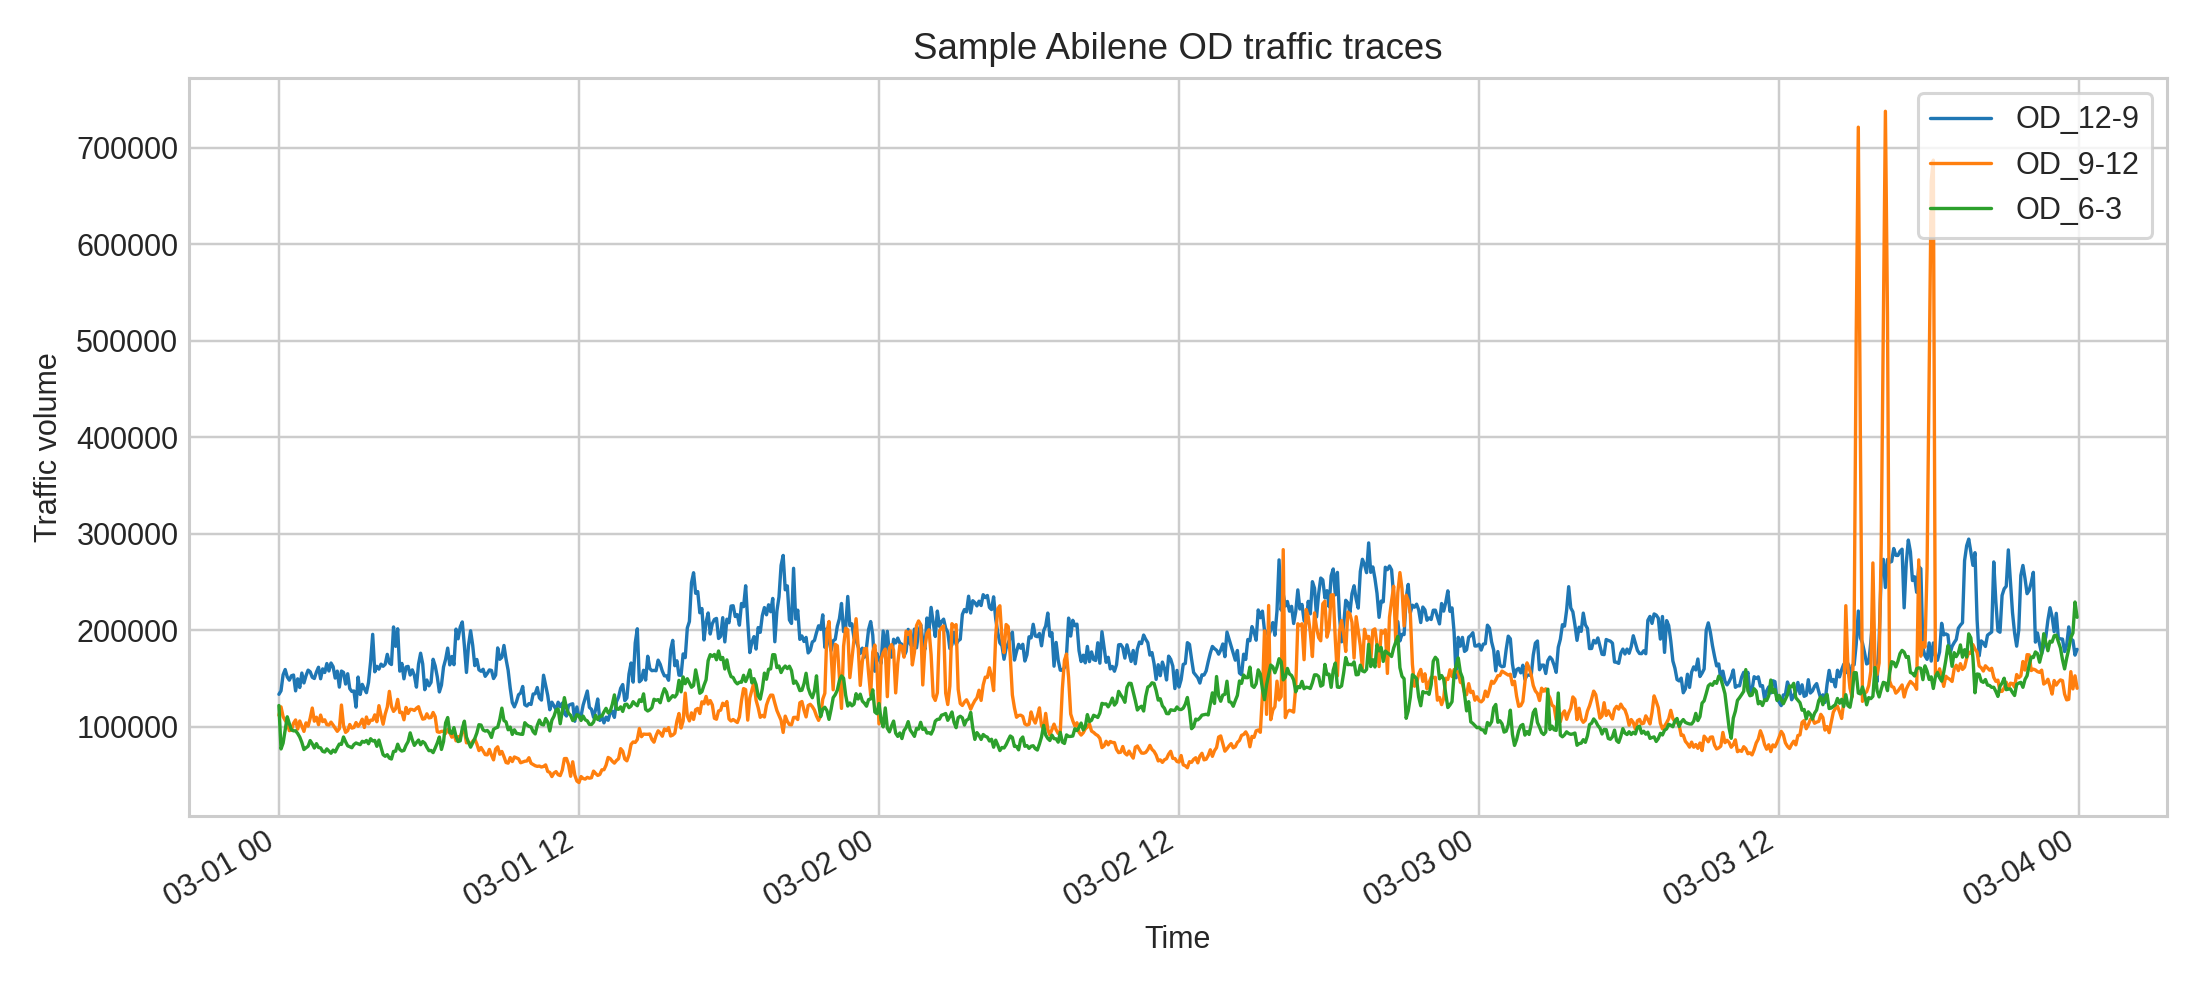
\includegraphics[width=0.9\linewidth]{traffic_sample.png}
  \caption{Representative high-volume Abilene OD traces from the sampled Protocol B dataset.}
  \label{fig:traffic-sample}
\end{figure}

\begin{figure}[h]
  \centering
  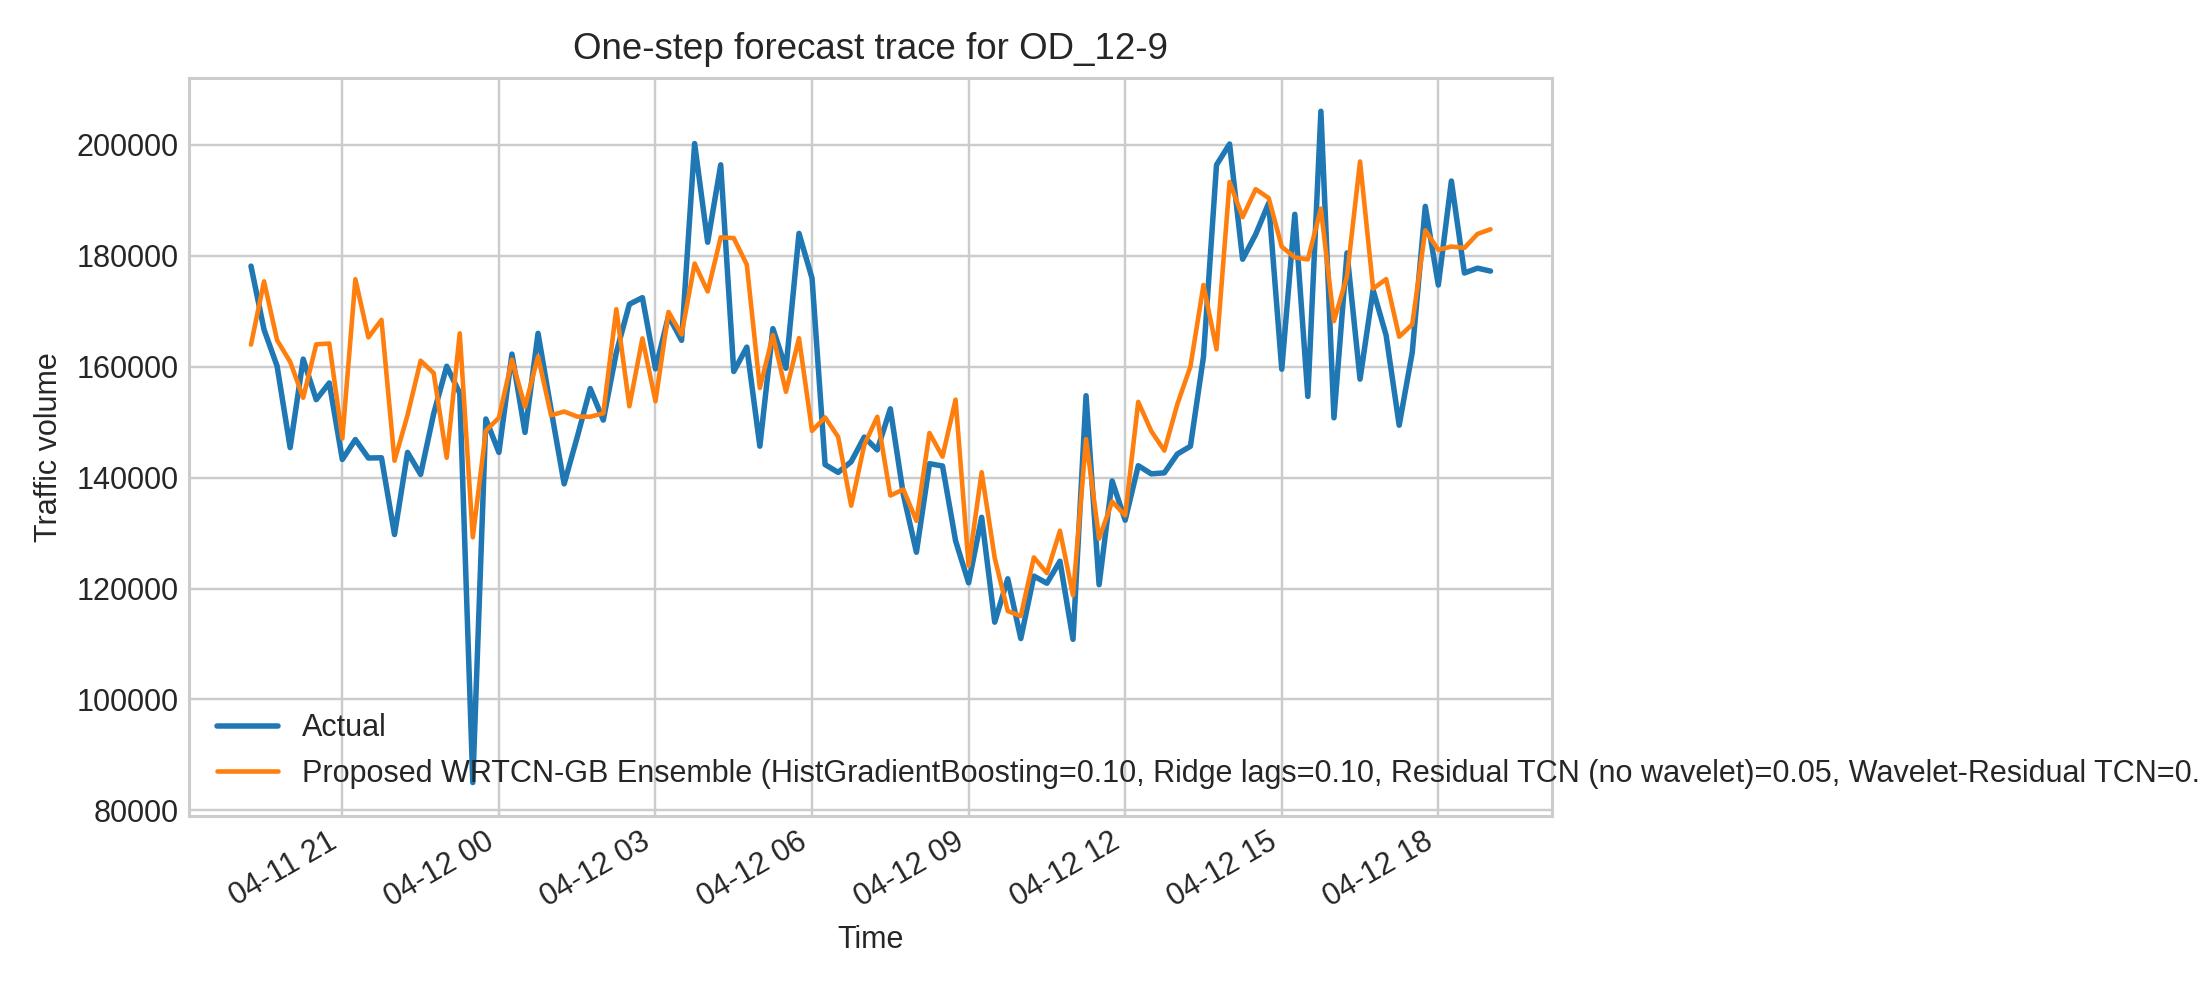
\includegraphics[width=0.9\linewidth]{prediction_trace.png}
  \caption{One-step forecast trace for a representative Protocol B test flow.}
  \label{fig:prediction-trace}
\end{figure}

\section*{NeurIPS Paper Checklist}

\begin{enumerate}
\item {\bf Claims}
    \item[] Question: Do the main claims made in the abstract and introduction accurately reflect the paper's contributions and scope?
    \item[] Answer: \answerYes{}.
    \item[] Justification: The abstract and introduction state bounded claims and explicitly avoid unconditional cross-paper SOTA claims.

\item {\bf Limitations}
    \item[] Question: Does the paper discuss the limitations of the work performed by the authors?
    \item[] Answer: \answerYes{}.
    \item[] Justification: The limitations and societal impact section discusses dataset age, cross-paper comparability, CPU-sized neural baselines, learned rather than physical graph attention, and the lack of physical-topology-aware graph evaluation.

\item {\bf Theory assumptions and proofs}
    \item[] Question: For each theoretical result, does the paper provide the full set of assumptions and a complete proof?
    \item[] Answer: \answerNA{}.
    \item[] Justification: The paper is empirical and does not present theoretical theorems or proofs.

\item {\bf Experimental result reproducibility}
    \item[] Question: Does the paper fully disclose all the information needed to reproduce the main experimental results?
    \item[] Answer: \answerYes{}.
    \item[] Justification: The data source, splits, metrics, hyperparameters, and exact reproduction commands are provided in the main paper and Appendix A.

\item {\bf Open access to data and code}
    \item[] Question: Does the paper provide open access to the data and code, with sufficient instructions to faithfully reproduce the main experimental results?
    \item[] Answer: \answerYes{}.
    \item[] Justification: The dataset is public and cited. The submission is intended to include anonymized code as supplementary material with the commands shown in Appendix A.

\item {\bf Experimental setting/details}
    \item[] Question: Does the paper specify all training and test details necessary to understand the results?
    \item[] Answer: \answerYes{}.
    \item[] Justification: Sections 4 and Appendix A specify datasets, splits, input lengths, horizons, selected flows where used, optimizer, loss, epochs, model sizes, Protocol C fold construction, and Protocol D neural settings.

\item {\bf Experiment statistical significance}
    \item[] Question: Does the paper report error bars suitably and correctly defined or other appropriate information about statistical significance?
    \item[] Answer: \answerYes{}.
    \item[] Justification: Protocol B reports 95\% bootstrap intervals for WAPE over unique forecast end timestamps. Protocol C reports three blocked chronological folds and fold-level bootstrap intervals. Protocol D reports blocked folds plus paired bootstrap deltas over shared forecast end timestamps.

\item {\bf Experiments compute resources}
    \item[] Question: For each experiment, does the paper provide sufficient information on compute resources needed to reproduce the experiments?
    \item[] Answer: \answerYes{}.
    \item[] Justification: The paper reports CPU execution, the CUDA failure condition, visible GTX 1050 hardware, and Protocol B/C/D runtimes.

\item {\bf Code of ethics}
    \item[] Question: Does the research conform to the NeurIPS Code of Ethics?
    \item[] Answer: \answerYes{}.
    \item[] Justification: The work uses public aggregate network traffic data, does not involve human subjects, and discusses possible misuse.

\item {\bf Broader impacts}
    \item[] Question: Does the paper discuss both potential positive and negative societal impacts?
    \item[] Answer: \answerYes{}.
    \item[] Justification: The limitations and societal impact section discusses operational efficiency benefits and possible traffic-monitoring misuse.

\item {\bf Safeguards}
    \item[] Question: Does the paper describe safeguards for responsible release of data or models with high misuse risk?
    \item[] Answer: \answerNA{}.
    \item[] Justification: The work does not release a high-risk generative model or scraped personal dataset; it uses public aggregate traffic matrices.

\item {\bf Licenses for existing assets}
    \item[] Question: Are original owners of assets used in the paper credited and are license or terms mentioned?
    \item[] Answer: \answerYes{}.
    \item[] Justification: The DL4Internet dataset repository is cited and its repository metadata reports an Apache-2.0 license, as stated in the data section.

\item {\bf New assets}
    \item[] Question: Are new assets introduced in the paper well documented and provided alongside the assets?
    \item[] Answer: \answerYes{}.
    \item[] Justification: The new code artifacts are documented by the reproduction commands and are suitable for anonymized supplementary release.

\item {\bf Crowdsourcing and research with human subjects}
    \item[] Question: For crowdsourcing experiments and research with human subjects, does the paper include full participant instructions and compensation details?
    \item[] Answer: \answerNA{}.
    \item[] Justification: The paper does not involve crowdsourcing or human subjects.

\item {\bf Institutional review board approvals}
    \item[] Question: Does the paper describe IRB approvals or equivalent for research with human subjects?
    \item[] Answer: \answerNA{}.
    \item[] Justification: The paper does not involve human subjects.

\item {\bf Declaration of LLM usage}
    \item[] Question: Does the paper describe LLM usage if it is an important, original, or non-standard component of the core method?
    \item[] Answer: \answerNA{}.
    \item[] Justification: LLMs are not part of the forecasting method, experiments, or core scientific contribution.
\end{enumerate}

\end{document}
